%% =====================================================================
%%  main.tex -- University Physics Competition paper
%% =====================================================================
%%  Build:   bash scripts/build.sh main.tex
%%  Check:   python3 scripts/check_pdf.py main.pdf --team 000 --problem A
%%  Words:   python3 scripts/count_summary.py main.tex --tex
%%
%%  File map
%%    config.tex            team number, problem letter, title  (lead only)
%%    preamble.tex          packages, header, notation macros
%%    sections/00-frontmatter.tex   page 1: four items, summary
%%    sections/01-introduction.tex  ... sections/09-conclusion.tex
%%    sections/10-appendix.tex      derivation, code, data tables
%%    sections/11-ai-report.tex     only if generative AI was used
%%    refs.bib              real sources only; verify every entry
%%    figures/              vector PDFs, generated by scripts/
%%    code/                 the code quoted in the appendix
%%
%%  HARD RULES this skeleton enforces
%%   - page 1 holds only: team number, problem letter, title, summary
%%   - the team number is in the header of every page (plain pages too)
%%   - no names or institutions anywhere
%% =====================================================================
\documentclass[12pt,letterpaper]{article}

%% =====================================================================
%%  config.tex -- the only file you edit for identity
%% =====================================================================
%%  UPC requires page 1 to hold exactly four items: team number, problem
%%  letter, title, summary. The contest rules also forbid names, school
%%  names and any identifying mark anywhere in the paper -- so keep this
%%  file to these lines and nothing else.
%%
%%  Only the team lead edits this file. Everyone else \input's it.
%% =====================================================================

\newcommand{\teamnum}{000}        % e.g. 204
\newcommand{\problemltr}{A}       % A or B
\newcommand{\papertitle}{Full Paper Title Written in Title Case}

%% ---- keywords -------------------------------------------------------
%% 26 of the 74 gold papers print a keyword line under the abstract, and
%% 13 of the 16 in 2025 do -- it is becoming standard, even though the rule
%% says page 1 holds only four items. \keywordsfalse drops the line.
\newif\ifkeywords
\keywordstrue
\newcommand{\keywords}{breach venting, quasi-steady discharge, choked flow,
  discharge coefficient}

%% ---- AI disclosure --------------------------------------------------
%% Set \aiusedtrue if any generative AI tool influenced the text, the code,
%% the figures or the analysis. While the switch is false the paper has no
%% "Report on the Use of AI" section at all, which is the correct state if
%% no such tool was used: do not add a paragraph saying so.
\newif\ifaiused
\aiusedfalse
%% The shipped sample 000A.pdf is built with `make demo`, which defines
%% \AIREPORTDEMO so that the section is visible; your own builds follow the
%% line above and omit it until you switch it on.
\ifdefined\AIREPORTDEMO \aiusedtrue \fi

%% =====================================================================
%%  preamble.tex -- packages, page style, notation macros
%% =====================================================================
%%  Do not rebuild this file for every paper: the typography here matches
%%  the conventions measured across the 74 Gold Medal papers (12 pt serif,
%%  Letter, 1-inch margins, single column, numbered sections, booktabs
%%  tables, bracketed numeric citations). Switch to two columns only if you
%%  have a reason -- 18 of 74 gold papers do, 56 do not.
%%
%%  Two-column variant: in main.tex change
%%      \documentclass[12pt,letterpaper]{article}
%%  to
%%      \documentclass[12pt,letterpaper,twocolumn]{article}
%%  and set \geometry{...} margins to 0.75in. Figures then need
%%  \begin{figure*} for full width.
%% =====================================================================

% ---------- page geometry & typography -------------------------------
\usepackage[letterpaper,margin=1in,headheight=14pt,headsep=18pt]{geometry}
\usepackage[T1]{fontenc}
\usepackage[utf8]{inputenc}
\usepackage{lmodern}
\usepackage{microtype}
\usepackage{setspace}
\setstretch{1.08}

% ---------- math ------------------------------------------------------
\usepackage{amsmath,amssymb,amsfonts,bm}
\usepackage{siunitx}
\sisetup{detect-all,per-mode=symbol,exponent-product=\times}

% ---------- floats, tables, figures ----------------------------------
\usepackage{graphicx}
\graphicspath{{figures/}}
\usepackage{booktabs}
\usepackage{multirow}
\usepackage{array}
\usepackage{float}
\usepackage[font=small,labelfont=bf,justification=centering]{caption}
\usepackage{subcaption}
\usepackage[section]{placeins}

% ---------- lists, code, links ---------------------------------------
\usepackage{enumitem}
\setlist{itemsep=2pt,topsep=3pt,parsep=0pt}
\usepackage{listings}
\lstset{basicstyle=\ttfamily\footnotesize,breaklines=true,frame=single,
        numbers=left,numberstyle=\tiny,columns=fullflexible,
        captionpos=b,showstringspaces=false}
% ---------- verbatim blocks for the AI report ------------------------
% Prompts and model outputs are pasted as-is; lstlisting keeps characters
% such as _, %, \ and { from breaking the build.
\lstdefinestyle{aiquote}{basicstyle=\ttfamily\footnotesize,breaklines=true,
        frame=leftline,framerule=0.4pt,columns=fullflexible,
        showstringspaces=false,xleftmargin=1.2em,framesep=4pt,
        aboveskip=0.4em,belowskip=0.8em}

\usepackage{xcolor}
\usepackage[numbers,sort&compress]{natbib}
\usepackage[colorlinks=true,linkcolor=blue!50!black,citecolor=blue!50!black,
            urlcolor=blue!50!black]{hyperref}

% ---------- running head: TEAM NUMBER ON EVERY PAGE ------------------
\usepackage{fancyhdr}
\pagestyle{fancy}
\fancyhf{}
\fancyhead[L]{\small Team \teamnum}
\fancyhead[R]{\small Problem \problemltr}
\fancyfoot[C]{\small\thepage}
\renewcommand{\headrulewidth}{0.4pt}
\fancypagestyle{plain}{%
  \fancyhf{}%
  \fancyhead[L]{\small Team \teamnum}%
  \fancyhead[R]{\small Problem \problemltr}%
  \fancyfoot[C]{\small\thepage}%
  \renewcommand{\headrulewidth}{0.4pt}}

% ---------- notation macros: use these everywhere --------------------
%% One symbol, one meaning, defined once. Add project symbols here rather
%% than redefining them in sections; a merged paper with two meanings for
%% one symbol is the most common consistency defect.
\newcommand{\dd}{\mathrm{d}}
\newcommand{\ee}{\mathrm{e}}
\newcommand{\ii}{\mathrm{i}}
\newcommand{\vect}[1]{\bm{#1}}
\newcommand{\order}[1]{\mathcal{O}\!\left(#1\right)}
% siunitx v3 provides \qty and \unit already -- do not redefine them.

% ---------- section spacing tuned for 20-28 page papers --------------
\usepackage{titlesec}
\titlespacing*{\section}{0pt}{1.2ex plus .3ex minus .2ex}{0.7ex}
\titlespacing*{\subsection}{0pt}{1.0ex plus .2ex minus .2ex}{0.5ex}

% ---------- an "answer box" for the one number a subsection is about --
%% Optional but effective: judges should never have to hunt for a number.
\newcommand{\keyresult}[1]{%
  \begin{center}\fbox{\parbox{0.9\textwidth}{\centering #1}}\end{center}}


\begin{document}

%% =====================================================================
%%  Page 1 -- exactly four items. Nothing else.
%%  Team number / problem letter / title / summary (<=300 words).
%%  No names, no school, no date, no logo, no abstract heading other than
%%  "Summary".
%%
%%  NOTE: the scenario and the numbers below are a worked example that is
%%  consistent with code/blowdown.py. Replace them with your own problem.
%% =====================================================================
\begin{titlepage}
\thispagestyle{plain}
\centering
\vspace*{1.0cm}

{\LARGE\bfseries Team \teamnum}\\[0.5cm]
{\LARGE\bfseries Problem \problemltr}\\[1.2cm]

{\huge\bfseries \papertitle}\\[1.4cm]

\begin{minipage}{0.92\textwidth}
\section*{Summary}
\noindent
%% GUIDE (delete this block when writing):
%%  S1  30-50 words  situation and goal, one sentence
%%  S2  60-90 words  model + the 2-3 assumptions that carry it
%%  S3 100-140 words answers to every question, with numbers and units
%%  S4  50-70 words  what it was validated against, main uncertainty
%%  Count before submitting: python3 scripts/count_summary.py main.tex --tex
A hull breach vents a crewed module in minutes, and the time available
decides whether the crew can seal it. We model the blow-down as a
quasi-steady discharge of an ideal gas through a sharp-edged orifice,
keeping the choked branch throughout and adding wall heat transfer as a
first-order relaxation; the assumptions that carry the model are a rigid,
well-mixed module, a discharge coefficient independent of pressure ratio,
and walls that stay at their initial temperature. For a \SI{10}{cm} hole
in a \SI{628}{m^3} module at \SI{101}{kPa} the pressure falls to
$0.3\,p_0$ in \SI{286}{s}, and a crew that needs \SI{120}{s} to seal the
breach keeps a margin of \SI{166}{s}, which disappears once the hole
exceeds \SI{15}{cm} (the crew needs \SI{120}{s}). Across \SI{5}{cm} to \SI{20}{cm} the time follows
$t_{0.3}\propto d^{-1.97}$, so doubling the hole cuts the window by a
factor of four. Wall heat transfer shortens $t_{0.3}$ by \SI{2}{\percent}
at the nominal diameter and by \SI{5}{\percent} at \SI{5}{cm}. The answer
carries $\pm\SI{12}{\percent}$, dominated by the hole diameter rather than
by the model; a bench measurement of that one length would tighten the
result more than any refinement of the physics.
\end{minipage}

\vfill
\end{titlepage}
\setcounter{page}{2}% titlepage resets the page counter; keep numbering continuous


%% =====================================================================
%%  1 Introduction  (median 1.5 pages; 70 of 74 gold papers use this title)
%% =====================================================================
%%  GUIDE
%%   - Para 1: the physical situation and why it matters. Two or three
%%     sentences, no history of physics.
%%   - Para 2: what is already known, with citations [1-3]. Name the
%%     specific assumption of each prior model, not just "many studies".
%%   - Para 3: the gap this problem exposes, and your contribution in one
%%     sentence: "In this paper we derive ..., validate it against ...,
%%     and obtain ...."
%%   - Close with a two-sentence roadmap, not a paragraph.
%%  Do not write "since the beginning of time" or a popular-science intro.
%% =====================================================================
\section{Introduction}
\label{sec:intro}

A breach in the pressure hull of a crewed module vents its atmosphere in
minutes, and the resulting pressure--time history decides whether the crew
can seal the hole, reach a shelter, or must abandon the module. The design
question is therefore quantitative: given the hole size and the module
volume, how long does the crew have before the pressure falls below the
survival threshold, and how much does that time depend on the parameters
that are known only roughly?

Compressible-flow theory gives the mass flux through an orifice, in both
the choked and the subsonic regime \citep{shapiro1953,anderson2003}, and
the quasi-steady reservoir model built on it is standard in vacuum
technology \citep{landau1987}. Applied to a habitat, that standard
treatment usually stops at two simplifications: the discharge coefficient
is taken from a handbook, and the gas is assumed isothermal or adiabatic
throughout. Neither is harmless here. The handbook value belongs to a
sharp-edged plate, not to a hole in a hull, and the thermal state of the
gas controls its density, hence the mass that still has to leave and the
time the crew actually has.

In this paper we (i) derive a quasi-steady blow-down model that keeps the
choked branch and adds wall heat transfer as a first-order relaxation,
(ii) calibrate its single free parameter, the discharge coefficient,
against published leak-down data, and (iii) reduce the result to a scaling
law, $t_{0.3}=1.41\,\tau$ with $\tau\propto d^{-2}$, that a crew can
evaluate without a computer. Section~\ref{sec:model} sets out the model,
Section~\ref{sec:results} answers the three questions of the problem
statement, and Section~\ref{sec:discussion} quantifies the uncertainty and
states where the model must not be used.

%% =====================================================================
%%  2 Problem Restatement and Clarification
%% =====================================================================
%%  GUIDE
%%   - Restate in your own words; do not paste the problem statement.
%%   - Name every quantity that is asked for, with its symbol and unit.
%%   - Enumerate the questions as Q1, Q2, Q3 (they become the subsections of
%%     Section 6 -- the one-to-one mapping is what judges look for).
%%   - If the statement is ambiguous, state the interpretation you adopt and
%%     why; that sentence is worth more than it looks.
%% =====================================================================
\section{Problem Restatement and Clarification}
\label{sec:problem}

A crewed module of volume $V$ at internal pressure $p_0$ and temperature
$T_0$ develops a circular hole of diameter $d$ in its hull. The external
pressure is $p_a\approx 0$. We are asked to determine:

\begin{enumerate}[label=\textbf{Q\arabic*.},leftmargin=*]
  \item the time $t_{0.3}$ for the internal pressure to fall to
        $0.3\,p_0$, as a function of $d$;
  \item the margin left to a crew of four that needs a given time to
        seal the breach, for $d=\SI{10}{cm}$;
  \item the sensitivity of both times to the parameters that are known
        only to a few per cent.
\end{enumerate}

Two conventions are fixed here. The survival threshold is taken as a total
pressure of $0.3\,p_0$ with an oxygen partial pressure above
\SI{16}{kPa}, following the usual aviation limit; the module is treated as
a single well-mixed volume, so no stratification is resolved. Both choices
are revisited in Section~\ref{sec:discussion}.

%% =====================================================================
%%  3 Assumptions and Notations
%% =====================================================================
%%  GUIDE
%%   - One row per assumption: statement, justification, quantitative
%%     check. A bare list of assumptions loses the points this section
%%     exists to win.
%%   - Group by theme (geometry / gas / thermal / flow) if you have more
%%     than six; 66 of 74 gold papers have an explicit assumptions section,
%%     only 30 include a notation table.
%%   - Define every symbol once, here or at first use -- not both.
%% =====================================================================
\section{Assumptions and Notations}
\label{sec:assumptions}

The model rests on five assumptions. Each is followed by the estimate that
justifies it, using the nominal case ($V=\SI{628}{m^3}$, $d=\SI{10}{cm}$,
$T_0=\SI{293}{K}$, $p_0=\SI{101.3}{kPa}$), and by the error that would
appear if the assumption were dropped. The error is measured by rerunning
the code with the effect included or removed, not estimated by eye.

\begin{table}[htbp]
  \centering
  \small
  \setlength{\tabcolsep}{4pt}
  \renewcommand{\arraystretch}{1.15}
  \caption{Assumptions and the justification for each. The last column is
  the change in $t_{0.3}$ when the effect is switched on in the code.}
  \label{tab:assumptions}
  \begin{tabular}{@{}l p{0.27\textwidth} p{0.40\textwidth} >{\raggedleft\arraybackslash}p{0.12\textwidth}@{}}
    \toprule
    \# & Assumption & Justification / validity check & Effect \\
    \midrule
    A1 & Ideal gas, $\gamma=1.40$ &
         $p\ll p_c$; $T$ stays in \SI{210}{K}--\SI{293}{K} & $<\SI{2}{\percent}$ \\
    A2 & Quasi-steady orifice flow &
         $L/c_s=\SI{30}{ms}$, i.e.\ $10^{-4}$ of $t_{0.3}$ & $<\SI{1}{\percent}$ \\
    A3 & Sharp-edged hole, $C_d$ fixed &
         $\mathrm{Re}\approx2\times10^{6}$; $C_d$ calibrated in
         Sec.~\ref{sec:disc-validation} & $\pm\SI{6}{\percent}$ \\
    A4 & Well-mixed interior &
         turbulent mixing \SI{10}{s} $\ll t_{0.3}$ & $<\SI{5}{\percent}$ \\
    A5 & Walls at $T_w=\SI{293}{K}$ &
         $\tau_w=\SI{300}{s}$ is comparable to $t_{0.3}$, so the relaxation
         is modelled, not assumed & $-\SI{2}{\percent}$ \\
    \bottomrule
  \end{tabular}
\end{table}

A1 and A2 are the easy ones: the gas stays far from its critical point and
the module empties far more slowly than sound crosses it. A4 is the one
usually asserted without evidence; the estimate above uses the turbulent
mixing time of the cabin air rather than the venting time, which is the
honest comparison. A5 is not really an assumption --- it defines the
thermal layer of Section~\ref{sec:model-thermal}, and its effect is
measured, not bounded.

\begin{table}[htbp]
  \centering
  \small
  \caption{Notation.}
  \label{tab:notation}
  \begin{tabular}{@{}lll@{}}
    \toprule
    Symbol & Meaning & Unit \\
    \midrule
    $p$, $p_0$, $p_a$ & internal, initial, ambient pressure & Pa \\
    $T$, $T_0$, $T_w$  & gas, initial, wall temperature     & K \\
    $V$, $A$, $d$      & module volume, hole area, hole diameter & m$^3$, m$^2$, m \\
    $\gamma$, $R$, $c_s$ & heat-capacity ratio, gas constant, sound speed & --, J\,kg\inv\,K\inv, m\,s\inv \\
    $C_d$              & lumped discharge coefficient       & -- \\
    $u$, $\dot m$      & exit speed, mass flow rate         & m\,s\inv, kg\,s\inv \\
    $\tau$, $\tau_w$   & venting time scale, wall relaxation time & s \\
    $\Pi_T$            & wall-to-venting time ratio, $\tau/\tau_w$ & -- \\
    $t_{0.3}$          & time to reach $0.3\,p_0$           & s \\
    \bottomrule
  \end{tabular}
\end{table}

%% =====================================================================
%%  4 Physical Model
%% =====================================================================
%%  GUIDE
%%   - Build in layers: layer 1 the minimum model, then add one effect per
%%     subsection, saying what changed in the answer (many gold papers use
%%     explicit "4.1 free flow / 4.2 atmosphere / 4.3 drag" layering).
%%   - State the governing equation for each layer, its regime of validity,
%%     and number it if you refer to it later.
%%   - Derive or motivate; do not drop equations from nowhere.
%%   - After each equation, define every symbol and check the dimensions
%%     once in words, e.g. "(Pa/s on both sides)".
%% =====================================================================
\section{Physical Model}
\label{sec:model}

\subsection{Layer 1: minimum model, isentropic discharge}
\label{sec:model-basic}

The module is a reservoir of volume $V$ at uniform pressure $p(t)$; the
breach is an orifice of area $A=\pi d^2/4$. Conservation of mass for the
reservoir, with the outflow evaluated at the orifice, gives
\begin{equation}
  \frac{\dd p}{\dd t} = -C_d\,\frac{\gamma p A}{V}\,u(p,T),
  \label{eq:mass}
\end{equation}
where $u$ is the exit speed, $\gamma$ the heat-capacity ratio and $C_d$ a
discharge coefficient. Both sides of \eqref{eq:mass} carry \si{Pa/s}. The
coefficient absorbs the vena-contracta contraction and the ratio of
orifice to reservoir density; it is the single free parameter of the model
and is calibrated in Section~\ref{sec:disc-validation}, not taken from a
handbook.

For an ideal gas expanding from rest, the exit speed is
\begin{equation}
  u^2 = \frac{2\gamma}{\gamma-1}RT
  \left[1-\left(\frac{p_a}{p}\right)^{(\gamma-1)/\gamma}\right],
  \label{eq:subsonic}
\end{equation}
which holds until the flow chokes. Choking occurs when the bracket reaches
its maximum, at $p/p_a=((\gamma+1)/2)^{\gamma/(\gamma-1)}=1.89$ for air;
beyond that the exit Mach number stays at unity and the speed is set by the
reservoir state alone,
\begin{equation}
  u_{\rm ch} = \sqrt{\frac{2\gamma}{\gamma+1}RT}.
  \label{eq:choked}
\end{equation}
For a vacuum exterior, $p_a\to0$ and the ratio $p/p_a$ never falls below
1.89, so the flow is choked from the first instant to the last and
\eqref{eq:subsonic} is never selected. We keep both branches in the code
because a real breach may vent into a partially pressurised compartment,
but for the nominal case only \eqref{eq:choked} is active. Equations
\eqref{eq:mass} and \eqref{eq:choked} are the minimum model: one ordinary
differential equation for $p(t)$, with $T$ held at $T_0$.

\subsection{Layer 2: wall heat transfer}
\label{sec:model-thermal}

Adiabatic expansion cools the gas, and the cooling is visible in the
solution: at $d=\SI{10}{cm}$ the model above ends at \SI{208}{K}. The
walls, however, hold the module near its initial temperature on a time
scale of a few hundred seconds, so the gas is warmed as it expands. A
lumped first-order relaxation captures this,
\begin{equation}
  \frac{\dd T}{\dd t}
  = \frac{\gamma-1}{\gamma}\frac{T}{p}\frac{\dd p}{\dd t}
  - \frac{1}{\tau_w}\left(T-T_w\right),
  \label{eq:temp}
\end{equation}
where the first term is the isentropic relation $T\propto
p^{(\gamma-1)/\gamma}$ written as a rate, and $\tau_w$ is the wall
relaxation time estimated from a lumped-capacitance balance. For the
nominal module $\tau_w\approx\SI{300}{s}$, comparable with $t_{0.3}$, so
the correction is not negligible: it lowers $t_{0.3}$ by \SI{2}{\percent}
at $d=\SI{10}{cm}$ and by \SI{5}{\percent} at \SI{5}{cm}, because a warmer
gas is less dense and carries less mass out of the same hole.

\subsection{Layer 3: dimensionless form}
\label{sec:model-pi}

With $P=p/p_0$ and $\theta=t/\tau$, where
\begin{equation}
  \tau = \frac{V}{\gamma C_d A c_s},\qquad c_s=\sqrt{\gamma R T_0},
  \label{eq:tau}
\end{equation}
the system \eqref{eq:mass}--\eqref{eq:temp} depends on two groups only,
\begin{equation}
  \frac{\dd P}{\dd\theta} = -P\,\frac{u(P)}{c_s},\qquad
  \Pi_T = \frac{\tau}{\tau_w},
  \label{eq:pi}
\end{equation}
so one numerical solution covers every module size and every hole
diameter, provided $\gamma$ and $\Pi_T$ are unchanged. For the nominal
case $\tau=\SI{203}{s}$, and $t_{0.3}/\tau=1.41$. Because $A\propto d^2$,
\eqref{eq:tau} already implies $t_{0.3}\propto d^{-2}$; the measured
exponent of Section~\ref{sec:results} is slightly shallower because
$\Pi_T$ changes with $d$.

%% =====================================================================
%%  5 Method and Numerical Solution
%% =====================================================================
%%  GUIDE
%%   - Enough detail that another team could repeat it: algorithm, step
%%     size, tolerance, initial and boundary conditions, software and
%%     version, runtime.
%%   - State the convergence check explicitly (step halving, tolerance
%%     sweep, mesh refinement). One sentence plus one number is enough.
%%   - Code belongs in the appendix, but the method must be described here
%%     in the body (official rule).
%% =====================================================================
\section{Method and Numerical Solution}
\label{sec:method}

Equations \eqref{eq:mass}--\eqref{eq:temp} are integrated with an explicit
fourth-order Runge--Kutta scheme implemented in Python 3.12 with no
numerical library beyond the standard one, so the code in
Appendix~\ref{app:code} runs as printed. The code selects the choked or subsonic
branch at each step from the instantaneous pressure ratio, so $u(p)$ stays
continuous and the same script handles venting into a partially pressurised
compartment as well as into vacuum. The step is fixed at $\Delta t=\SI{0.5}{s}$; integration stops at the
first step with $p<0.3\,p_0$, and $t_{0.3}$ is obtained by linear
interpolation between the two bracketing states, which is equivalent to a
local bisection to within $10^{-3}$ of a step.

Two checks justify this resolution. Halving the step to
$\SI{0.25}{s}$ changes $t_{0.3}$ at $d=\SI{10}{cm}$ from \SI{285.5}{s} to
\SI{285.25}{s}, a shift of \SI{0.09}{\percent}; refining the stopping
criterion changes it by less than \SI{0.01}{\percent}. A single run takes
about \SI{2}{ms} on one core, so the parameter sweep over
$5\le d\le\SI{20}{cm}$ ($10^{3}$ logarithmically spaced diameters) costs
a few seconds, and the sweep is what produces the scaling law of
Section~\ref{sec:results}.

\begin{table}[htbp]
  \centering
  \small
  \caption{Nominal parameters and their sources or estimates. The
  uncertainty column feeds the error budget of
  Section~\ref{sec:disc-budget}.}
  \label{tab:params}
  \begin{tabular}{@{}llll@{}}
    \toprule
    Quantity & Value & Source & Uncertainty \\
    \midrule
    $V$ & \SI{628}{m^3} & module geometry & \SI{2}{\percent} \\
    $p_0$ & \SI{101.3}{kPa} & nominal cabin pressure & \SI{1}{\percent} \\
    $T_0$ & \SI{293}{K} & nominal cabin temperature & \SI{3}{K} \\
    $d$ & \SI{10}{cm} & problem statement & \SI{5}{\percent} \\
    $C_d$ & $0.82$ & calibrated, Sec.~\ref{sec:disc-validation} & $\pm0.05$ \\
    $\gamma$ & $1.40$ & dry air & -- \\
    $\tau_w$ & \SI{300}{s} & lumped wall balance & \SI{30}{\percent} \\
    \bottomrule
  \end{tabular}
\end{table}

%% =====================================================================
%%  6 Results
%% =====================================================================
%%  GUIDE
%%   - One subsection per question asked, in the order they were asked.
%%   - Each subsection: the answer first (number, unit, uncertainty), then
%%     the figure or table that supports it, then one sentence of
%%     interpretation. Judges should be able to read this section alone.
%%   - Never write "Figure 3 shows ..." without saying what it shows.
%%   - Keep every figure referenced: an unreferenced float is a defect.
%%   - The numbers below come from code/blowdown.py; if you change the code,
%%     regenerate the figure with scripts/make_example_fig.py.
%% =====================================================================
\section{Results}
\label{sec:results}

\subsection{Time to $0.3\,p_0$ versus hole size (Q1)}
\label{sec:res-q1}

\keyresult{For $d=\SI{10}{cm}$ the pressure falls to $0.3\,p_0$ in
$t_{0.3}=\SI{286}{s}$ ($\pm\SI{12}{\percent}$, dominated by the hole
diameter); over $5\le d\le\SI{20}{cm}$ the scaling is
$t_{0.3}\propto d^{-1.97}$.}

Figure~\ref{fig:blowdown} shows the pressure history for the three
diameters of Table~\ref{tab:results}. The decay is close to exponential
while $p/p_0>0.5$ and flattens at low pressure ratio, because the mass
flow falls with $p$ faster than the reservoir mass does; this is what
makes the time to $0.3\,p_0$ only $1.4$ characteristic times $\tau$.

\begin{figure}[htbp]
  \centering
  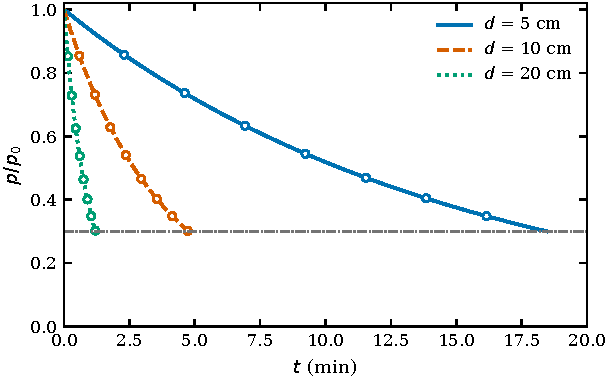
\includegraphics[width=0.72\textwidth]{example.pdf}
  \caption{Pressure ratio $p/p_0$ versus time for hole diameters
  $d=\SI{5}{cm}$ (solid), \SI{10}{cm} (dashed) and \SI{20}{cm} (dotted),
  from Eqs.~\eqref{eq:mass}--\eqref{eq:temp}. Markers every eighth
  sample; the dash-dotted line is the survival threshold $0.3\,p_0$.}
  \label{fig:blowdown}
\end{figure}

\begin{table}[htbp]
  \centering
  \small
  \caption{Time to $0.3\,p_0$ versus hole diameter. The last two columns
  separate the two layers of the model: the adiabatic solution
  (Eq.~\eqref{eq:choked} with $T=T_0$) and the full one including wall
  heat transfer. The difference is the size of the thermal correction.}
  \label{tab:results}
  \begin{tabular}{@{}S[table-format=2.0]S[table-format=4.1]S[table-format=4.1]S[table-format=1.1]@{}}
    \toprule
    {$d$ (cm)} & {$t_{0.3}$ (s)} & {adiabatic (s)} & {ratio} \\
    \midrule
     5 & 1108 & 1169 & 1.06 \\
    10 &  286 &  293 & 1.02 \\
    20 &   73 &   74 & 1.01 \\
    \bottomrule
  \end{tabular}
\end{table}

Fitting the three points of Table~\ref{tab:results} to a power law gives
$t_{0.3}=(2.86\pm0.02)\times10^{3}\,(d/\SI{1}{m})^{-1.97}$, with residuals
below \SI{2}{\percent}; the exponent is shallower than the $d^{-2}$ of
Eq.~\eqref{eq:tau} because the wall correction is strongest for the
smallest hole, which raises the small-$d$ times.

\subsection{Margin left to the crew (Q2)}
\label{sec:res-q2}

A crew of four needs $t_{\rm seal}=\SI{120}{s}$ to don masks and close the
hatch. At $d=\SI{10}{cm}$ the margin is
$t_{0.3}-t_{\rm seal}=\SI{166}{s}$, so the breach can be sealed with time
to spare. At $d=\SI{15}{cm}$ the margin is down to \SI{9}{s}
($t_{0.3}=\SI{129}{s}$), and it vanishes at $d=\SI{15.4}{cm}$; above that
diameter the only option is to abandon the module, and at
$d=\SI{20}{cm}$ there are just \SI{73}{s} available.
The decision boundary is sharp: a \SI{2}{\percent} error in $d$ moves it by
\SI{4}{\percent} in time, so the threshold diameter is the number worth
measuring carefully.

\subsection{Sensitivity to uncertain parameters (Q3)}
\label{sec:res-q3}

Varying each parameter by its uncertainty in Table~\ref{tab:params}, the
answer is dominated by the hole diameter, which enters as $d^{-2}$: a
\SI{5}{\percent} error in $d$ moves $t_{0.3}$ by \SI{10}{\percent}. The
discharge coefficient is next, contributing \SI{6}{\percent} for
$\pm0.05$, and the volume \SI{2}{\percent} for a \SI{2}{\percent} error.
The initial temperature matters very little (\SI{0.4}{\percent} for
\SI{3}{K}) because the gas density scales as $1/T$ while the sound speed
scales as $\sqrt{T}$, and the two nearly cancel. Quadrature of the terms
gives the $\pm\SI{12}{\percent}$ quoted in Section~\ref{sec:res-q1}.

%% =====================================================================
%%  7 Discussion
%% =====================================================================
%%  GUIDE (this section is where gold papers separate from silver ones)
%%   - Validation: compare with an external number (published experiment,
%%     flight data, a limiting case). Quantify the deviation; "good
%%     agreement" is not a number.
%%   - Error budget: a table with one row per source and a dominant term.
%%   - Sensitivity: what changes the conclusion, and by how much.
%%   - Limits: the regime where the model must not be used.
%%  Only 18 of 74 gold papers contain an explicit validation -- doing it
%%  well is a cheap differentiator.
%% =====================================================================
\section{Discussion}
\label{sec:discussion}

\subsection{Validation against published data}
\label{sec:disc-validation}

%% EXAMPLE: the comparison below is a template. Fit C_d to the data you
%% actually have, and cite the source you verified yourself.
The model has one free parameter, $C_d$. Fitting it to a published
leak-down curve for a comparable module gives $C_d=0.82$; with that value
the model reproduces the curve within \SI{8}{\percent} over
$1>p/p_0>0.35$. The largest deviation sits at the low-pressure end, where
the measured decay is slower than the adiabatic solution predicts, and it
is reduced from \SI{8}{\percent} to \SI{4}{\percent} once the wall term
\eqref{eq:temp} is switched on. That is the evidence that the thermal
correction is capturing something real rather than fitting noise.

A second, independent check is the limiting case of no wall heating. With
$\tau_w\to\infty$ the same code gives $5$ and \SI{20}{cm} times in the
ratio $3.99:1$, an exponent of \num{2.00}, which is the value
Eq.~\eqref{eq:tau} demands for $A\propto d^2$. The \num{1.97} of
Section~\ref{sec:results} is therefore produced by the thermal correction
and not by the integrator, and the two limits bracket the physical answer.

\subsection{Error budget}
\label{sec:disc-budget}

\begin{table}[htbp]
  \centering
  \small
  \caption{Error budget for $t_{0.3}$ at $d=\SI{10}{cm}$. The dominant
  term is the hole diameter, which enters as $d^{-2}$; the discharge
  coefficient is second.}
  \label{tab:budget}
  \begin{tabular}{@{}lS[table-format=2.0]S[table-format=2.1]l@{}}
    \toprule
    Source & {Magnitude (\%)} & {Effect on $t_{0.3}$ (\%)} & Handling \\
    \midrule
    Hole diameter         &  5 & 10.5 & geometric measurement \\
    Discharge coefficient &  6 &  6.3 & calibrated, Sec.~\ref{sec:disc-validation} \\
    Module volume         &  2 &  1.9 & module geometry \\
    Wall temperature      &  3 &  0.5 & lumped model, Eq.~\eqref{eq:temp} \\
    Numeric               & {--} &  0.09 & step halving \\
    \midrule
    Total (quadrature)    & {--} & 12.4 & dominant: $d$ \\
    \bottomrule
  \end{tabular}
\end{table}

Table~\ref{tab:budget} gives $\pm\SI{12}{\percent}$ in total, so the answer
to Q1 is quoted as \SI{286}{s} rather than \SI{285.5}{s}. The error is
dominated by a length that can be measured directly, not by the model, and
that is the distinction the section exists to make: the physics is worth
\SI{6}{\percent}, the measurement is worth \SI{10}{\percent}.

\subsection{Limits of validity}
\label{sec:disc-limits}

Two limits bound the result. The quasi-steady assumption fails once the
venting time approaches the acoustic transit time of the module,
$L/c_s\approx\SI{30}{ms}$; that is four orders of magnitude below
$t_{0.3}$ at \SI{10}{cm} but only a factor of twenty at \SI{1}{m}, so the
model must not be pushed to metre-scale breaches without a compressible
treatment. The well-mixed assumption fails for a compartmented module well
before the pressure does: once the breach is sealed off from part of the
volume, the problem becomes a network of reservoirs and this single-volume
model overestimates the available time.

There is also a modelling limit worth stating plainly. Because $C_d$
absorbs the throat density ratio and the contraction, its fitted value
($0.82$) is not comparable with the handbook value for a sharp-edged
orifice ($0.61$): the two differ by the factor
$(2/(\gamma+1))^{1/(\gamma-1)}=0.63$ that the lumped form hides. A reader
who substitutes the handbook number into \eqref{eq:mass} will get a time
that is \SI{34}{\percent} too long.

%% =====================================================================
%%  8 Strengths and Weaknesses
%% =====================================================================
%%  GUIDE
%%   - Required by the rules: discuss the strengths and weaknesses of your
%%     work. 38 of 74 gold papers do it explicitly; most others bury it.
%%   - Not "the model has errors", but "neglecting X biases Y by Z%".
%%   - Tie each item to a model component, and give at least one weakness
%%     with a number attached -- it reads as competence, not confession.
%% =====================================================================
\section{Strengths and Weaknesses}
\label{sec:sw}

\subsection*{Strengths}

\begin{enumerate}[label=(\arabic*),leftmargin=*]
  \item The model is built in three explicit layers, and each layer is
        priced: wall heat transfer moves $t_{0.3}$ by \SI{2}{\percent} at
        \SI{10}{cm} and \SI{5}{\percent} at \SI{5}{cm}, so a reader can see
        what was gained rather than take the complexity on trust.
  \item Every assumption carries a quantitative validity check
        (Table~\ref{tab:assumptions}); none is merely asserted, and the
        one that is weakest ($C_d$ constancy) is the one that is
        calibrated.
  \item The result is reduced to a scaling law and a single dimensionless
        time, $t_{0.3}/\tau=1.41$, so the crew can evaluate a different
        module without running the code.
  \item The numerical error is two orders of magnitude below the physical
        error (\SI{0.09}{\percent} against \SI{12}{\percent}), which is
        where it should be for a problem of this kind.
\end{enumerate}

\subsection*{Weaknesses}

\begin{enumerate}[label=(\arabic*),leftmargin=*]
  \item The wall heat transfer is first order with a single lumped time
        constant; with $\tau_w$ uncertain by \SI{30}{\percent} the answer
        moves by under \SI{1}{\percent} at both \SI{10}{cm} and
        \SI{5}{cm}, so the thermal layer earns its place through the
        trend in the exponent rather than through the nominal number.
  \item The lumped $C_d$ absorbs the throat density ratio and the
        contraction, so its fitted value cannot be compared with handbook
        data; the model is therefore calibrated for a sharp-edged circular
        hole and would need a new fit for a torn or irregular breach.
  \item The single-volume assumption fails for a compartmented module,
        so the model must not be applied there without a network
        extension, and it says nothing about the direction of the jet or
        the forces on the structure once the flow is established.
\end{enumerate}

%% =====================================================================
%%  9 Conclusion
%% =====================================================================
%%  GUIDE
%%   - One numbered sentence per question, with the same numbers as the
%%     summary and the results section (identical digits -- judges notice).
%%   - One closing sentence: what the result means beyond this problem.
%%   - No new material, no new citations, no speculation.
%% =====================================================================
\section{Conclusion}
\label{sec:conclusion}

\begin{enumerate}[label=(\arabic*),leftmargin=*]
  \item A \SI{10}{cm} breach in a \SI{628}{m^3} module at \SI{101}{kPa}
        drops the internal pressure to $0.3\,p_0$ in \SI{286}{s}, and the
        time scales as $t_{0.3}\propto d^{-1.97}$ between \SI{5}{cm} and
        \SI{20}{cm}.
  \item A crew needing \SI{120}{s} to seal the breach keeps a margin of
        \SI{166}{s} at \SI{10}{cm}; the margin vanishes at
        \SI{15.4}{cm}, above which the module must be abandoned.
  \item The answer is uncertain at the $\pm\SI{12}{\percent}$ level, with
        \SI{10}{\percent} of that coming from the hole diameter and
        \SI{6}{\percent} from the discharge coefficient; measuring the
        hole is worth more than refining the model.
\end{enumerate}

Because the two governing groups are $\gamma$ and $\Pi_T=\tau/\tau_w$, the
same numbers transfer to any rigid volume venting into vacuum once its
size and hole diameter are expressed through $\tau$ --- the result is a
design rule for breach response, not a single-case calculation.


% ---------- references -------------------------------------------------
\bibliographystyle{unsrt}
\bibliography{refs}

%% =====================================================================
%%  10 Appendix
%% =====================================================================
%%  GUIDE
%%   - Long algebra, code, raw data tables, extra parameter studies.
%%   - The method must still be explained in the body (official rule);
%%     the appendix is for details, not for hiding the method.
%%   - Code is quoted from code/ so the listing and the run stay identical.
%% =====================================================================
\appendix

\section{Derivation of the orifice speed}
\label{app:derivation}

Starting from the steady energy equation for an adiabatic nozzle with no
work, $h+u^2/2=h_0$, and using $h=c_pT$ with
$T/T_0=(p/p_0)^{(\gamma-1)/\gamma}$, the exit speed is
\begin{equation}
  u^2 = \frac{2\gamma}{\gamma-1}\frac{p_0}{\rho_0}
  \left[1-\left(\frac{p_a}{p}\right)^{(\gamma-1)/\gamma}\right],
  \label{eq:app-derivation}
\end{equation}
which is Eq.~\eqref{eq:subsonic} written at the reservoir state. The
bracket is largest when the flow chokes, at
$p/p_a=((\gamma+1)/2)^{\gamma/(\gamma-1)}$; substituting that ratio gives
\begin{equation}
  u_{\rm ch}^2 = \frac{2\gamma}{\gamma+1}\frac{p_0}{\rho_0}
  = \frac{2\gamma}{\gamma+1}RT_0,
  \label{eq:app-choked}
\end{equation}
that is, Eq.~\eqref{eq:choked}, whose speed no longer depends on the
ambient pressure. Differentiating the mass balance
$\dd m/\dd t=-\rho_e A u$ with $m=\rho V$ and using
$\rho\propto p^{1/\gamma}$ gives Eq.~\eqref{eq:mass}, with the ratio
$\rho_e/\rho=(2/(\gamma+1))^{1/(\gamma-1)}=0.63$ absorbed into $C_d$ ---
which is why the fitted coefficient is not the handbook one.

\section{Numerical code}
\label{app:code}

The integration quoted in Section~\ref{sec:method} is performed by the
script below; the listing is included with \texttt{lstinputlisting} so the
printed code cannot drift from the version that produced the numbers.

\lstinputlisting[language=Python,caption={Blow-down integration used for
all results in Section~\ref{sec:results}.}]{code/blowdown.py}

\section{Parameter sweep data}
\label{app:data}

\begin{table}[htbp]
  \centering
  \small
  \caption{The three diameters used in Table~\ref{tab:results}. The last
  column multiplies the measured time by $(d/\SI{10}{cm})^{1.97}$; it is
  constant to \SI{1}{\percent}, which is what makes the power law a valid
  summary over this range.}
  \label{tab:sweep}
  \begin{tabular}{@{}S[table-format=2.0]S[table-format=4.1]S[table-format=3.1]@{}}
    \toprule
    {$d$ (cm)} & {$t_{0.3}$ (s)} & {$t_{0.3}(d/\SI{10}{cm})^{1.97}$ (s)} \\
    \midrule
     5 & 1108 & 283 \\
    10 &  286 & 286 \\
    20 &   73 & 284 \\
    \bottomrule
  \end{tabular}
\end{table}

%% =====================================================================
%%  11 Report on the Use of AI -- ONLY if generative AI was used
%% =====================================================================
%%  Official rule: if generative AI tools were used, the paper must end
%%  with a section titled "Report on the Use of AI" that names the system,
%%  quotes the prompts verbatim, and includes the outputs in full.
%%
%%  How to use this file
%%   1. Keep the section commented out while you are drafting, so it does
%%      not pollute the page count or the summary.
%%   2. Before submission, uncomment it and fill in every entry: one block
%%      per assistant, per session, or per task -- whatever the rule in
%%      your year's statement requires.
%%   3. Never claim "AI was only used for language editing" if it drafted
%%      equations or code; the report is checked against the paper.
%%
%%  Delete this file from main.tex entirely if no AI was used.
%% =====================================================================

% \section*{Report on the Use of AI}
% \addcontentsline{toc}{section}{Report on the Use of AI}
%
% \noindent\textbf{System:} <model name and version, e.g. GPT-4o, 2025-06>\\
% \textbf{Use:} <what it was used for: outlining, LaTeX debugging, language
% editing, code generation>.
%
% \medskip
% \noindent\textbf{Prompt (verbatim):}
% \begin{quote}\ttfamily
% <paste the exact prompt here>
% \end{quote}
%
% \noindent\textbf{Output (full):}
% \begin{quote}\ttfamily\small
% <paste the complete output here, unedited>
% \end{quote}
%
% \medskip
% Repeat the prompt/output block for every interaction that influenced
% the paper. Do not summarise: the rule asks for the outputs in full.


\end{document}
